% Experiment 2: three square graphs plus the posterior of a and b
% for Different slopes and intercepts. Same format as Experiment 1.
\begin{figure}[H]
\centering
\rule{\textwidth}{0.4pt}\\[3pt]
\setlength{\tabcolsep}{0pt}
\begin{tabular}{@{}cccc@{}}
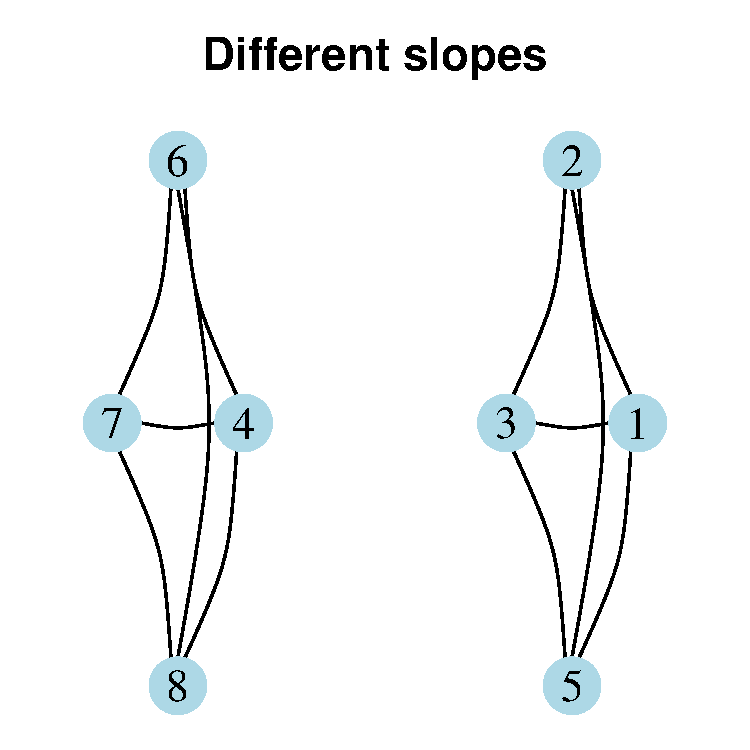
\includegraphics[width=4cm,height=4cm]{fig_experiment2_a_different_slopes.pdf} &
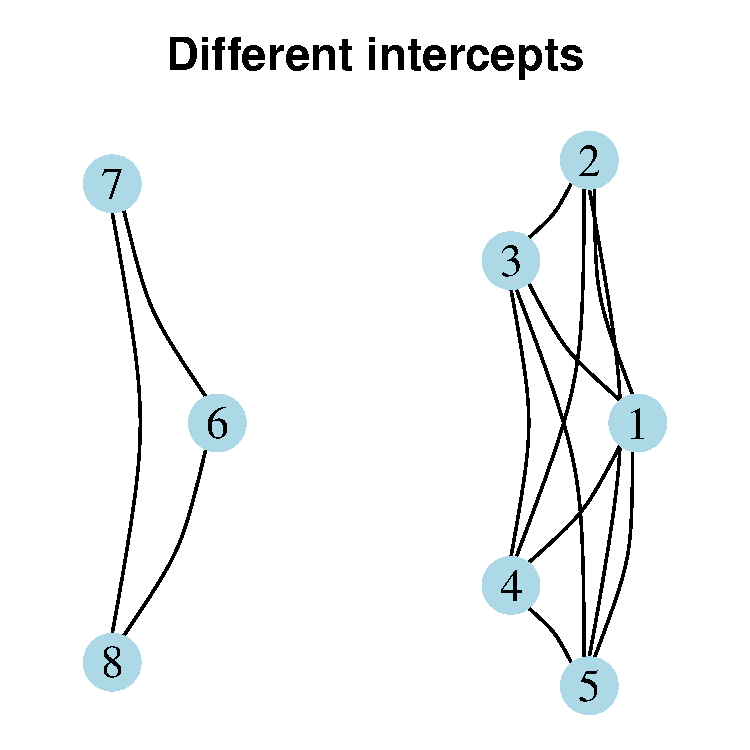
\includegraphics[width=4cm,height=4cm]{fig_experiment2_b_different_intercepts.pdf} &
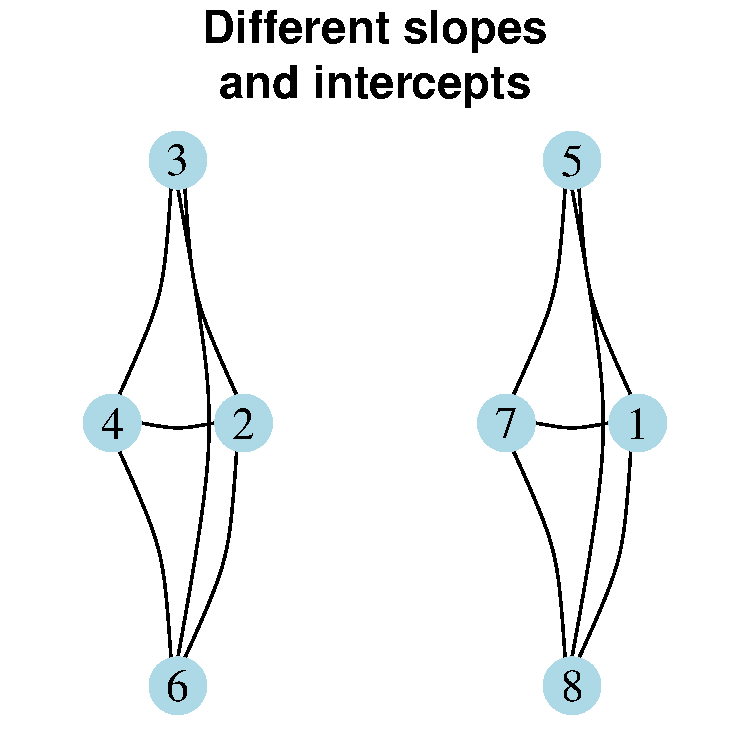
\includegraphics[width=4cm,height=4cm]{fig_experiment2_c_different_slopes_and_intercepts.pdf} &
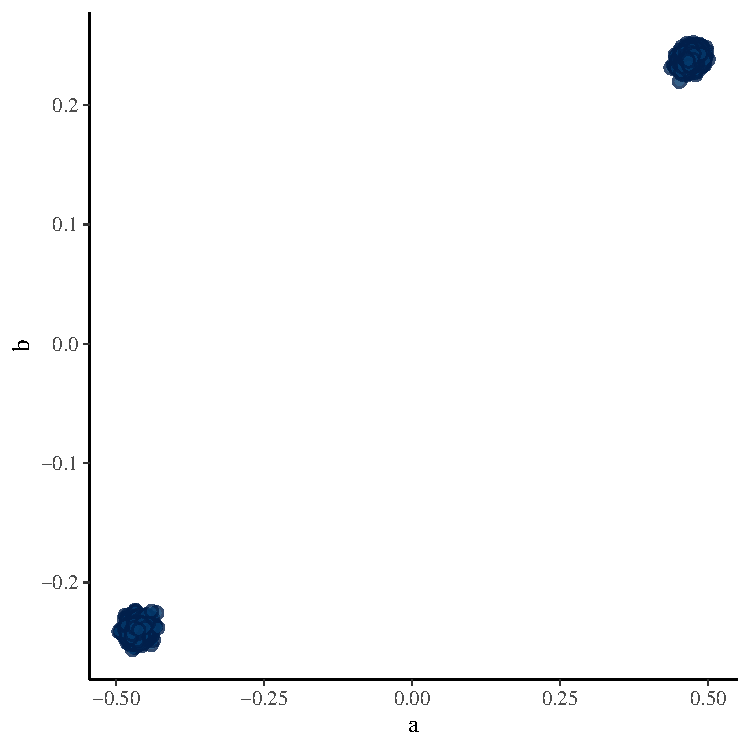
\includegraphics[width=4cm,height=4cm]{fig_experiment2_d_posterior_a_b.pdf}
\end{tabular}\\[3pt]
\rule{\textwidth}{0.4pt}
\caption{%
\textbf{MCMC convergence graphs for the three Experiment~2 models,
and the joint posterior of $a$ and $b$ for Different slopes and intercepts.}
The first three panels are intersection graphs $G_\cap$.
}
\label{fig:experiment2-graphs}
\end{figure}
